\documentclass[final]{beamer}
% beamer 3.10: do NOT use option hyperref={pdfpagelabels=false} !
% \documentclass[final,hyperref={pdfpagelabels=false}]{beamer} 
% beamer 3.07: get rid of beamer warnings

\mode<presentation> {  
%% check http://www-i6.informatik.rwth-aachen.de/~dreuw/latexbeamerposter.php for examples
  \usetheme{Durham} %% This points to the theme cooked up by the final year tutor
}


\usepackage{siunitx}
\usepackage[english]{babel} 
\usepackage[latin1]{inputenc}
\usepackage{amsmath,amsthm, amssymb, latexsym}

  \usefonttheme[onlymath]{serif}
  \boldmath
  \usepackage[orientation=portrait,size=a0,scale=1.4,debug]{beamerposter}                       

  % e.g. for DIN-A0 poster
  % \usepackage[orientation=portrait,size=a1,scale=1.4,grid,debug]{beamerposter}
  % e.g. for DIN-A1 poster, with optional grid and debug output
  % \usepackage[size=custom,width=200,height=120,scale=2,debug]{beamerposter} % e.g. for custom size poster
  % \usepackage[orientation=portrait,size=a0,scale=1.0,printer=rwth-glossy-uv.df]{beamerposter}
  % e.g. for DIN-A0 poster with rwth-glossy-uv printer check ...
  %

  \title[Final Year Project Poster]{Enigma and BOMBE Simulation}
  \author[A L Gillies]{Alexander Gillies}
  \institute[Durham]{School of Engineering and Computing Sciences, Durham University}
  \date{16th April 2012}

  \begin{document}
  \begin{frame}{} 

  \vfill
    \begin{columns}[t]
    
%%%%%%%%%%%%%%%%%%%%%%%%%%%%%%%%%%%%%%%%%%%      
    
      \begin{column}{.32\linewidth}
      \centering
        \begin{block}{Enigma}
          The Enigma is an electromechanical device that was the main force behind the impressive interconnectivity available to the Axis powers throughout the second world war.
        \end{block}
        
         \begin{block}{Antique Enigma}
          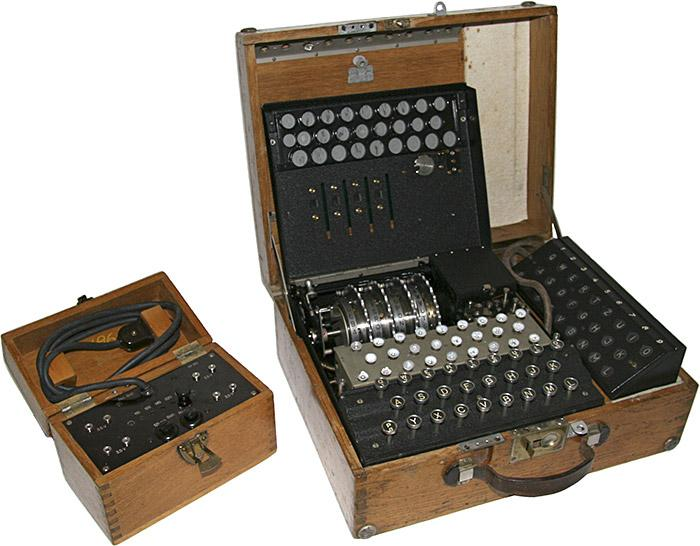
\includegraphics[width=.5\columnwidth]{historicEnigma.png} 
        \end{block}
        
         \begin{block}{History} \small{
          The Enigma is the brainchild of  Arthur Scherbius at the end of the First World War, the first uses were purely commercial. In February of 1918 Mr Scherbius along with E. Richard Ritter applied for a patent for a machine that used rotors for the purposes of encryption. This was the first implementation of the Enigma. The Enigma has many different versions, this includes the version that was used by the German Navy also known as the M3. The M3 incorperates three of the patented rotors that were the hallmark of the machine. The machine aesthetically was very similar to a large typewriter. M3 has a keyboard that was used as an input for the message to be encrypted, and a light-board to show the encrypted letter. The settings used by the network of machines was sent to all operators and they would then set up the machine by selecting the three rotors in the order they would be placed into the machine, they would reprogram the plug-board and the reflector. Once the machine was set up it was possible to encrypt and decrypt message that were send using the settings provided.}
        \end{block}
        
        \begin{block}{Technical Diagram of the Enigma}
          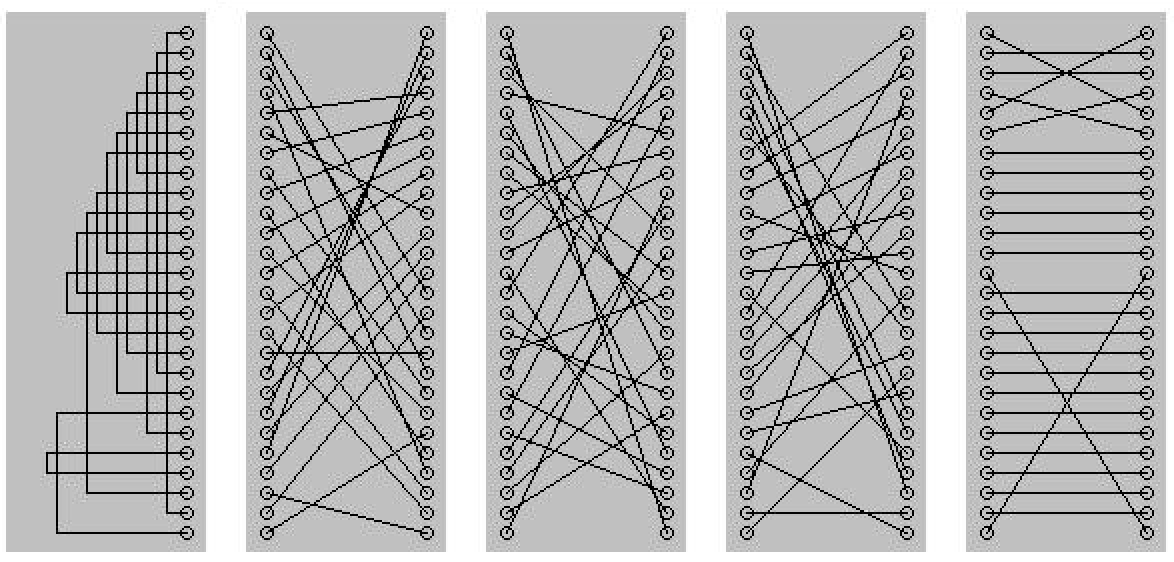
\includegraphics[width=\columnwidth]{enigma.png} 
        \end{block}
        
         \begin{block}{Technical}
          \begin{itemize} \small{
          \item The M3 is made up of a plug-board, three rotors and a reflector.
          \item The plug-board is a simple mapping between two alphabets, but is also reprogrammable.
          \item The rotors are stepping mapping between two alphabets that feed into the following rotor.
          \item The reflector is very similar to the plug-board and feeds its output back into the third rotor for the return journey.
          \item The whole system comes together in the form of a letter being input into the plug-board, which will then map from the input alphabet to the one specified by the settings of the plug-board, then these will be input into the first of the three rotors, this will perform another mapping, output into the second rotor, another mapping, input into the third rotor which would then output to the reflector. The reflector in another static mapping that will not change until the settings used for each day are changed, unlike the rotors which change mapping with each letter of the message that is input. Once the reflector has mapped its input then the output it put back into the third rotor but is mapped in the opposite direction and this is then done again in the second and first rotors, in that order. Finally the letter is returned through the plug-board, and output to the light-board.}
          \end{itemize}
        \end{block}

      \end{column}

%%%%%%%%%%%%%%%%%%%%%%%%%%%%%%%%%%%%%%%%%%%      

      \begin{column}{.32\linewidth}
      \centering
       \begin{block}{BOMBE}
          The BOMBE was an electromechanical device used by the British with help from the Polish to break the Enigma codes during the Second World War.
        \end{block}
        
        \begin{block}{A historic photograph of the BOMBE}
          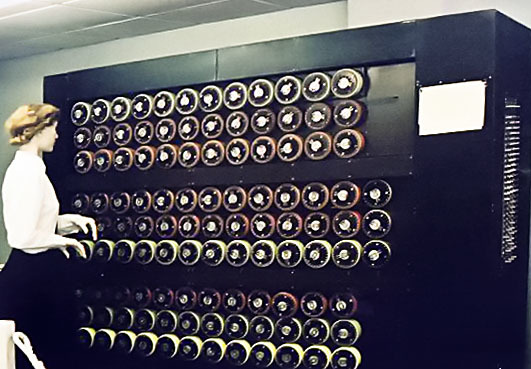
\includegraphics[width=\columnwidth]{historicBOMBE.png} 
        \end{block}
        
        \begin{block}{History} \small{
		First conceptualised by Polish cryptographer Marian Rejewski as part of the Biuro Szyfr\'ow or Cipher Bureau in 1938. Know as the bomba kryptologiczna or cryptologic bomb. This was the first stage of the breaking of the Enigma, in 1939 a revised and much improved version was proposed by Alan Turing, with another breakthrough being made by Gordon Welchman in 1940. The mechanical engineering and construction work was done by Harold Keen of the British Tabulating Machine Company.}
        \end{block}
        
         \begin{block}{The cabling of the BOMBE}
          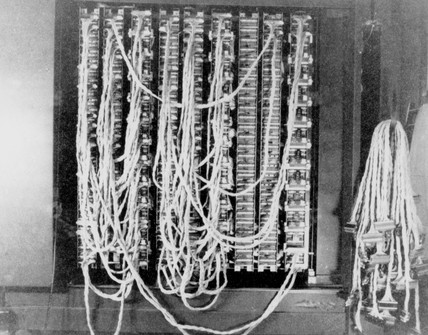
\includegraphics[width=\columnwidth]{bombeCable.png} 
        \end{block}
        
        \begin{block}{Technical}
          \begin{itemize}\small{
          \item Made up of three banks of 12 rows of three rotor representations.
          \item The BOMBE was was made to be a representation of the core of the Enigma, meaning the three rotors and reflector. Each bank would be wired to test a specific setting and would stop if the setting was tested to be correct. This test was done by a component known as a diagonal-board that was developed by Gordon Welchman.
          \item The rotor that is representing position one of the Enigma rotated at a speed of 120rpm, and each subsequent rotor at 1/26th the speed of its predecessor.
          \item Once a "Stop" had been reached, meaning that the settings had been tested and was a possible match to the settings used by the German forces that day, then frequency analysis would be done on the result to verify that these were the correct settings.}
          \end{itemize}
        \end{block}

      \end{column}
      
 %%%%%%%%%%%%%%%%%%%%%%%%%%%%%%%%%%%%%%%%%%%      
      
      \begin{column}{.32\linewidth}
        \begin{block}{Parallel Techniques}
          The idea of doing multiple things at once has always been a dream of people everywhere. It is called parallel programming in computers an has been possible for quite a few years.
        \end{block}
        
        \begin{block}{History}
          The idea of Multiple Instructions Multiple Data, or truly independent parallel programming was discussed in 1958 by S. Gill and also by IBM researchers John Cocke and Daniel Slotnick in the same year. The first processor that was capable of parallel programming was introduced in 1962 by the Burroughs Corporation in the form of the D825. Single Instruction Multiple Dataset processors such as the D825 can be traced from around this time, the first true commercial processors were not available until nearer to the turn of the century with AMD and Intel releasing their first multicore processors to the public around the same time.
        \end{block}
        
        \begin{block}{SIMD and MIMD}
          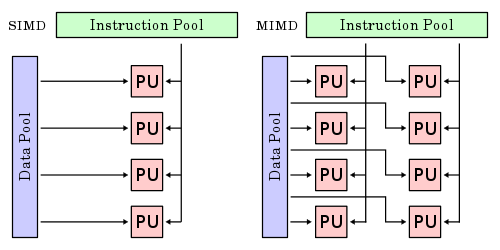
\includegraphics[width=\columnwidth]{parallel.png} 
        \end{block}
        
        \begin{block}{Technical}
          \begin{itemize}
          \item The idea of the MIMD system is doing different instructions on different sets of data.
          \item The idea of the SIMD system is doing the same instructions on multiple different pieces of data, also known as vector processing.
          \item The MIMD architecture is based around the concept of separate cores that each have separate memory but also have shared memory in which most of the data is stored, with a set of rules that dictate how this memory is accessed and written to between the cores.
          \item The SIMD architecture used vectorised loads, the idea that more than once data item can have an operation applied to it in one go.
          \end{itemize}
        \end{block}
        
	\begin{block}{Problem Decomposition}
          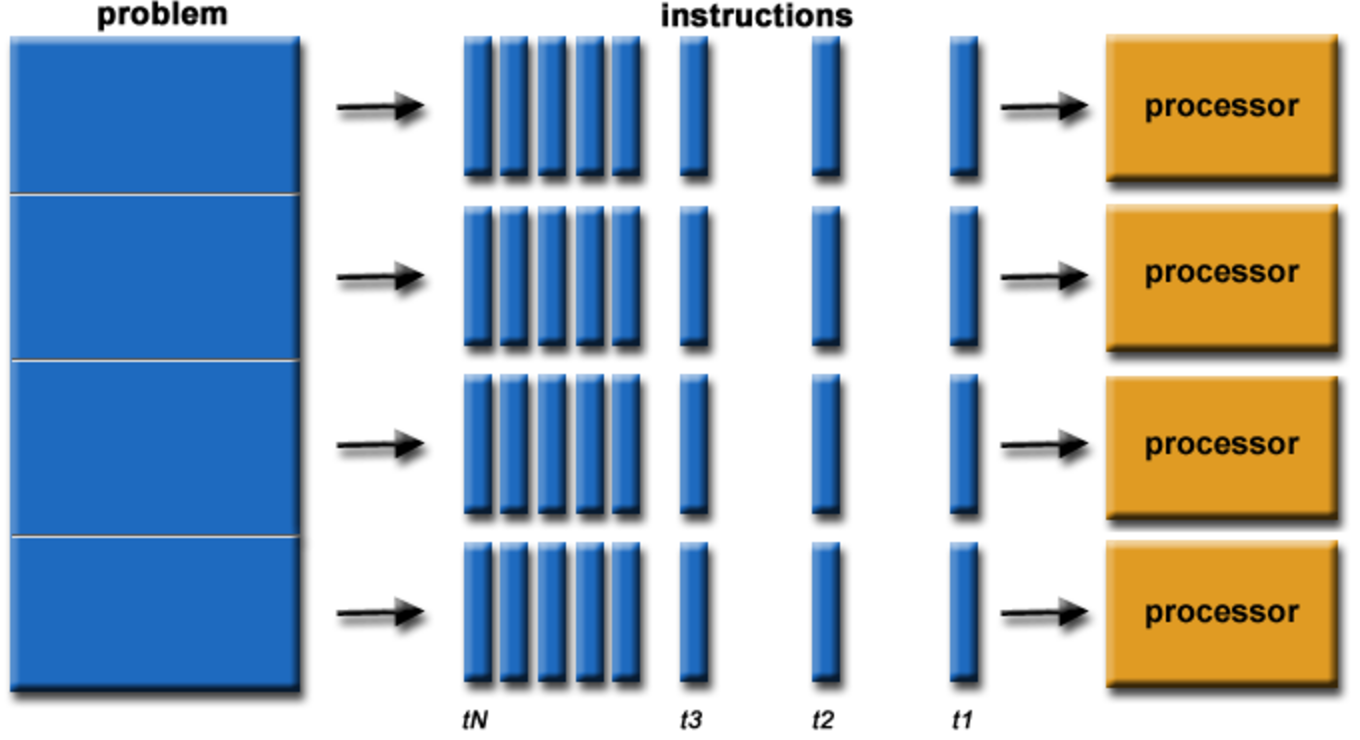
\includegraphics[width=\columnwidth]{problemDecomp.png} 
        \end{block}

      \end{column}      
      
%%%%%%%%%%%%%%%%%%%%%%%%%%%%%%%%%%%%%%%%%%%  
      
    \end{columns}

  \vfill
    \begin{block}{\centering Results}
		The time taken by the historic version of the BOMBE decrypted a 20 letter ciphertext in roughly 14400 seconds or roughly 4 hours. The time taken for a brute force version of the BOMBE implemented on a modern processor takes \num{6.12e47} or roughly \num{6e40} years. The recreation version of the BOMBE takes 48.22 seconds and the improved parallel version only took on average 17.62 seconds to break the enigma code.
    \end{block}
    \vfill

  \end{frame}
\end{document}


